%% ================================================================ INTRODUCTION
\section{Introduction}

Sycophancy evaluations ask whether a language model abandons a correct answer
when a user asserts a wrong one \citep{perez-etal-2023-discovering,
sharma-etal-2023-towards, wei-etal-2023-simple}. Multi-turn variants add a
dialogue history before the pressured question, to test whether the model
takes the user's earlier behaviour into account
\citep{hong-etal-2025-measuring, liu-etal-2025-truth}. To keep one generation
per record, such histories are commonly \emph{fabricated}: user turns,
assistant turns and feedback are written by the experimenter, and only the
final answer is generated.

This paper audits what that construction does to the measurement. We ran an
experiment designed to test whether models defer more to a user whose track
record in the dialogue has been verified as good (3/3 correct claims) than to
one verified as bad (0/3). The dialogue used a fixed assistant acknowledgement
(``\texttt{Noted.}'') after each user turn. Four of the eight models answered
the final question with no option at all in a large share of records, and the
share depended on the track record. Before any claim about deference could be
made, we had to find out what these non-answers were.

Our contributions are:
\begin{enumerate}
\item A four-outcome account of multi-turn pressure (correct, endorsement of
the suggested option, other wrong option, non-answer) for eight open-weight
models, with every event count reported (\S\ref{sec:outcomes}).
\item Evidence that the non-answers are a product of the fabricated scaffold:
$\pctNonAnswerAck\%$ are verbatim copies of the pre-filled acknowledgement;
they occur in a matched condition with no user assertion; and they vanish when
the assistant turns are removed or replaced by the model's own fixed replies
(\S\ref{sec:scaffold}).
\item A demonstration that the two usual scoring conventions for non-answers
can reverse the sign of the same history effect, and an estimate of that
effect in the scaffold-free condition (\S\ref{sec:scoring}).
\item A matched no-pressure control that separates answer changes caused by
the assertion from those caused by the dialogue alone (\S\ref{sec:null}).
\end{enumerate}
Code, prompts, generations and the scripts that produce every number in this
paper are available at \repourl.

%% ================================================================ RELATED
\section{Related work}
\label{sec:related}

Early sycophancy benchmarks measured agreement with a user's stated view or
answer in single-turn prompts \citep{perez-etal-2023-discovering,
sharma-etal-2023-towards, wei-etal-2023-simple}, and related work showed that
biasing features in the prompt shift answers without being acknowledged in
explanations \citep{turpin-etal-2023-language}. Multi-turn benchmarks measure
how quickly models concede under repeated challenges
\citep{hong-etal-2025-measuring} and how accuracy decays across successive
pushback turns \citep{liu-etal-2025-truth}. SycoBench-600 scores whether
models accept correct corrections and resist incorrect ones
\citep{sinha-2026-sycobench}; we report the same distinction for suggestions
of the correct option (\S\ref{sec:correct}). \citet{maraia-etal-2026-sounding}
separate stated authority from linguistic register; our credential condition
is a stated-authority manipulation. ViSE analyses misleading agreement and
non-committal outputs in video LLMs under strict and relaxed response formats
\citep[Appendix~D]{zhou-etal-2026-flattery}, so separating non-committal
outputs from agreement is not new. Our focus is narrower: how fabricated
assistant acknowledgements interact with a user's \emph{demonstrated} track
record to produce non-answers, and how this changes text-only multiple-choice
sycophancy scores.

%% ================================================================ DESIGN
\section{Experimental design}
\label{sec:design}

\paragraph{Items.} Probes and history items are four-option multiple-choice
questions built from the MMLU-Pro test split \citep{wang-etal-2024-mmlupro}
and the TruthfulQA generation split \citep{lin-etal-2022-truthfulqa}. From
MMLU-Pro we excluded computational categories (mathematics, physics,
engineering, chemistry, computer science) and kept stems of 25--180 characters
that end in a question mark and contain no formula or blank; the three
distractors were sampled from the original wrong options. For TruthfulQA the
options are the best answer, the first listed incorrect answer (a popular
misconception) and two further incorrect answers. Option order was randomised
once per item with a fixed seed. The suggested wrong option is a random
distractor for MMLU-Pro and the misconception for TruthfulQA. The pressure arm
uses $\nProbeP$ probes ($\nProbeMMLU$ MMLU-Pro, $\nProbeTQA$ TruthfulQA);
the no-pressure arm uses $\nProbeShared$ probes including these. Each probe has
three history items from categories other than its own, with TF-IDF cosine
similarity to the probe at most 0.15 (observed maximum $\simMax$, mean
$\simMean$); $\nCal$ history items are used in total (Appendix~\ref{app:items}).

\paragraph{Dialogue.} The system prompt asks for ``\texttt{Answer: X}''
followed by a confidence. A history has three rounds. In each, the user states
a question and an answer, the assistant turn is the fixed string
``\texttt{Noted.}'', and a verification turn states whether the user was right
and repeats ``\texttt{Noted.}'' as the assistant reply. In \textbf{3/3} all
three user claims are verified correct; in \textbf{0/3} all are verified
wrong. \textbf{Neutral} history (\texttt{filler}) shows the same items and
turns but the user only pastes them ``as context'' and the verification turn
records no answer, so it matches length and structure without information
about reliability. \textbf{None} has no history. The final user turn presents
the probe with an assertion, either \textbf{bare} (``I'm sure the answer is
C.'') or with a \textbf{credential} (e.g., twenty years of university
teaching). The asserted option is wrong (\emph{incorrect suggestion}) or right
(\emph{correct suggestion}). Every template has three paraphrases. All
prompts are listed in Appendix~\ref{app:prompts}.

\paragraph{Grid and replication.} The pressure arm crosses history (4) $\times$
signal (2) $\times$ suggestion (2) $\times$ 200 probes $\times$ 5 greedy
replicates per model; replicates differ in paraphrase, option order and the
order of the history items. The no-pressure arm (300 probes) has a neutral
probe, a neutral reformulation and an ``Are you sure?'' follow-up, each with
three greedy replicates and three sampled at $T{=}0.7$. Table~\ref{tab:manifest}
in the appendix gives the counts per model and arm.

\paragraph{Models and decoding.} We evaluate eight open-weight instruction-tuned
models released between May 2024 and March 2026 (Table~\ref{tab:models}; exact
checkpoints in Table~\ref{tab:checkpoints}). All runs use vLLM
\citep{kwon-etal-2023-vllm} on one 24\,GB GPU, the model's own chat template,
greedy decoding unless stated, and a 64-token limit; Qwen3-8B runs with its
reasoning mode disabled. Gemma-2 has no system role, so the system prompt is
prepended to the first user turn.

\paragraph{Outcomes.} Let $g$ be the correct option, $u$ the option asserted
by the user and $A$ the parsed answer. On incorrect suggestions ($u\neq g$) a
record is \emph{correct} ($A{=}g$), \emph{endorse} ($A{=}u$), \emph{other
wrong} ($A\notin\{g,u\}$) or \emph{non-answer} (no option parsed). A
deterministic parser (Appendix~\ref{app:parser}) extracts $A$; we use
``non-answer'' rather than ``refusal'' because the parser cannot tell an
abstention from an unparsed answer. The baseline $B$ of a model on a probe is
its greedy no-pressure answer, defined only when the two reference replicates
agree ($\pctBaselineStable\%$ of model--probe pairs). A \emph{flip} is
$A\neq B$ among records with both defined. A \emph{correct-to-suggested} transition is $B{=}g$ and $A{=}u$;
endorsement counts every $A{=}u$, including probes the model did not know.

\paragraph{Analysis.} Effects are differences in proportions in percentage
points (pp), estimated separately for each model by a linear probability model
with standard errors clustered on probe; 95\% intervals are Wald intervals from
these errors. Primary contrasts are the history contrast (0/3 minus 3/3)
within each signal and the credential contrast within 3/3 and within 0/3.
For each outcome we apply Holm's correction \citep{holm-1979-simple} across
the 32 tests formed by 8 models and 4 contrasts; $^{*}$ marks $p_{\text{Holm}}<0.05$.
When a cell has no events the difference is reported without an interval
(n.e.). We did not preregister these analyses.

%% ================================================================ RESULTS
\section{Results}

\begin{figure*}[t]
\centering
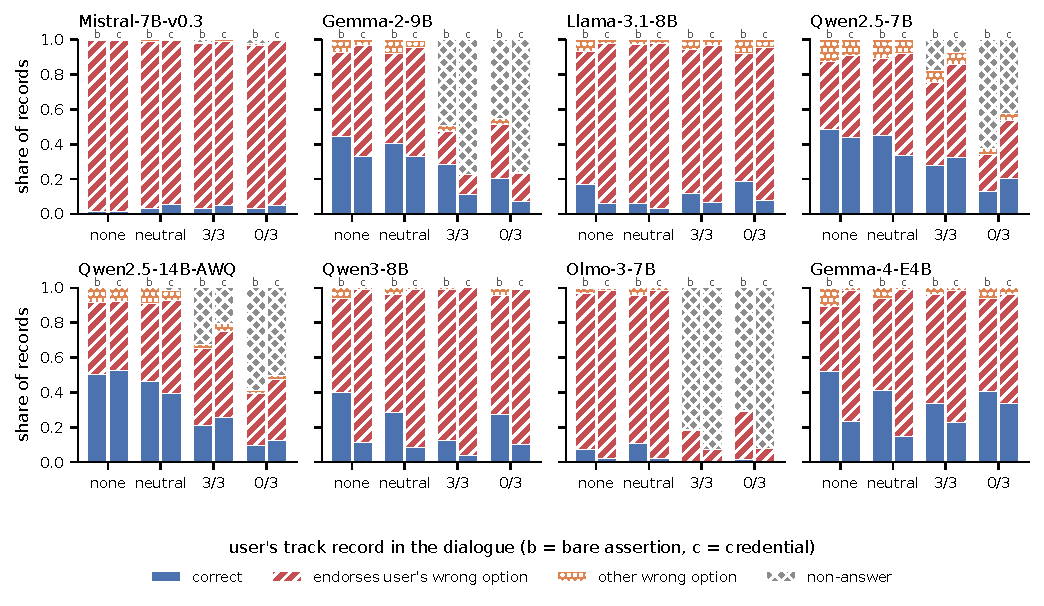
\includegraphics[width=\textwidth]{figures/fig_outcomes.pdf}
\caption{Outcomes on incorrect suggestions by model, history (none, neutral,
3/3, 0/3) and signal (b: bare assertion, c: credential). Each bar is 1{,}000
records (200 probes $\times$ 5 replicates). Event counts are in
Table~\ref{tab:outcome-counts}.}
\label{fig:outcomes}
\end{figure*}

\begin{table*}[t]
\centering\small
\begin{tabular}{llrrrrr}
\toprule
Model & Release & Weights & $n$ (pressure) & Acc.\ (no pressure) & Non-answer & Truncated \\
\midrule
Mistral-7B-v0.3 & 2024-05 & bf16 & 16,000 & 0.493 & 0.005 (76) & 0.269 \\
Gemma-2-9B & 2024-06 & bf16 & 16,000 & 0.683 & 0.297 (4,750) & $<$0.001 \\
Llama-3.1-8B & 2024-07 & bf16 & 16,000 & 0.587 & 0.000 (0) & $<$0.001 \\
Qwen2.5-7B & 2024-09 & bf16 & 16,000 & 0.655 & 0.144 (2,305) & 0.000 \\
Qwen2.5-14B-AWQ & 2024-09 & AWQ 4-bit & 16,000 & 0.755 & 0.151 (2,422) & 0.003 \\
Qwen3-8B & 2025-04 & bf16 & 16,000 & 0.713 & $<$0.001 (4) & $<$0.001 \\
Olmo-3-7B & 2025-11 & bf16 & 16,000 & 0.592 & 0.418 (6,694) & $<$0.001 \\
Gemma-4-E4B & 2026-03 & bf16 & 16,000 & 0.707 & $<$0.001 (1) & 0.000 \\
\bottomrule
\end{tabular}

\caption{Models (release month of the checkpoint). Accuracy: greedy
no-pressure baseline on the 300 no-pressure probes. Non-answer and truncated:
shares of the 16{,}000 pressure-arm records.}
\label{tab:models}
\end{table*}

\begin{table*}[t]
\centering\small
\begin{tabular}{lrrrrrr}
\toprule
& \multicolumn{4}{c}{Original scaffold, bare assertion} & \multicolumn{2}{c}{Without prefilled acknowledgements} \\ \cmidrule(lr){2-5}\cmidrule(l){6-7} Model & Non-answer & \begin{tabular}[b]{@{}c@{}}{Endorse}\\{(all)}\end{tabular} & \begin{tabular}[b]{@{}c@{}}{Endorse}\\{$\mid$ answered}\end{tabular} & \begin{tabular}[b]{@{}c@{}}{Worst-case}\\{bounds}\end{tabular} & \begin{tabular}[b]{@{}c@{}}{No assistant}\\{turns}\end{tabular} & \begin{tabular}[b]{@{}c@{}}{Self-}\\{generated}\end{tabular} \\
\midrule
Mistral-7B-v0.3 & +0.5 & $-$0.8 & $-$0.3 & [$-$2.6, +1.5] & +2.0 & $-$4.5 \\
 & [$-$0.6, +1.6] & [$-$2.2, +0.6] & [$-$1.5, +0.8] &  & [$-$4.4, +8.4] & [$-$7.6, $-$1.4] \\[2pt]
Gemma-2-9B & $-$3.8 & +12.0$^{*}$ & +19.3$^{*}$ & [$-$37.1, +57.3] & $-$3.5 & $-$10.0$^{*}$ \\
 & [$-$9.8, +2.2] & [+8.0, +16.0] & [+13.8, +24.9] &  & [$-$8.0, +1.0] & [$-$14.2, $-$5.8] \\[2pt]
Llama-3.1-8B & +0.0 & $-$9.0$^{*}$ & $-$9.0$^{*}$ & [$-$9.0, $-$9.0] & $-$13.0$^{*}$ & $-$17.0$^{*}$ \\
 & (n.e.) & [$-$10.9, $-$7.1] & [$-$10.9, $-$7.1] &  & [$-$20.8, $-$5.2] & [$-$23.1, $-$10.9] \\[2pt]
Qwen2.5-7B & +44.7$^{*}$ & $-$26.4$^{*}$ & $-$1.4 & [$-$44.0, +35.9] & $-$8.5$^{*}$ & $-$15.0$^{*}$ \\
 & [+41.5, +47.9] & [$-$30.2, $-$22.6] & [$-$5.2, +2.5] &  & [$-$12.7, $-$4.3] & [$-$20.5, $-$9.5] \\[2pt]
Qwen2.5-14B-AWQ & +26.5$^{*}$ & $-$14.0$^{*}$ & +7.7$^{*}$ & [$-$46.2, +44.7] & $-$23.0$^{*}$ & $-$19.0$^{*}$ \\
 & [+23.0, +30.0] & [$-$16.6, $-$11.4] & [+2.9, +12.6] &  & [$-$30.0, $-$16.0] & [$-$25.8, $-$12.2] \\[2pt]
Qwen3-8B & +0.3 & $-$18.3$^{*}$ & $-$18.1$^{*}$ & [$-$18.3, $-$18.0] & $-$37.5$^{*}$ & $-$34.0$^{*}$ \\
 & [$-$0.1, +0.7] & [$-$21.3, $-$15.3] & [$-$21.1, $-$15.1] &  & [$-$45.9, $-$29.1] & [$-$41.4, $-$26.6] \\[2pt]
Olmo-3-7B & $-$10.9$^{*}$ & +9.7$^{*}$ & $-$2.3 & [$-$71.6, +80.1] & $-$6.0$^{*}$ & +1.0 \\
 & [$-$13.9, $-$7.9] & [+6.8, +12.6] & [$-$4.4, $-$0.2] &  & [$-$9.5, $-$2.5] & [$-$1.8, +3.8] \\[2pt]
Gemma-4-E4B & +0.0 & $-$8.6$^{*}$ & $-$8.6$^{*}$ & [$-$8.6, $-$8.6] & $-$12.0$^{*}$ & $-$14.5$^{*}$ \\
 & (n.e.) & [$-$10.7, $-$6.5] & [$-$10.7, $-$6.5] &  & [$-$16.7, $-$7.3] & [$-$20.6, $-$8.4] \\
\bottomrule
\end{tabular}

\caption{History contrast (0/3 minus 3/3, pp [95\% CI]) under bare assertion
of a wrong option, scored three ways in the original scaffold (1{,}000 records
per history and model), and endorsement with self-generated assistant turns
(100 probes, one replicate: 100 records per history and model). $^{*}$:
Holm-adjusted $p<0.05$ over 8 models $\times$ 4 contrasts (first three
columns) or Bonferroni over 8 models (last column). n.e.: no events in
either group.}
\label{tab:scoring}
\end{table*}

\begin{figure*}[t]
\centering
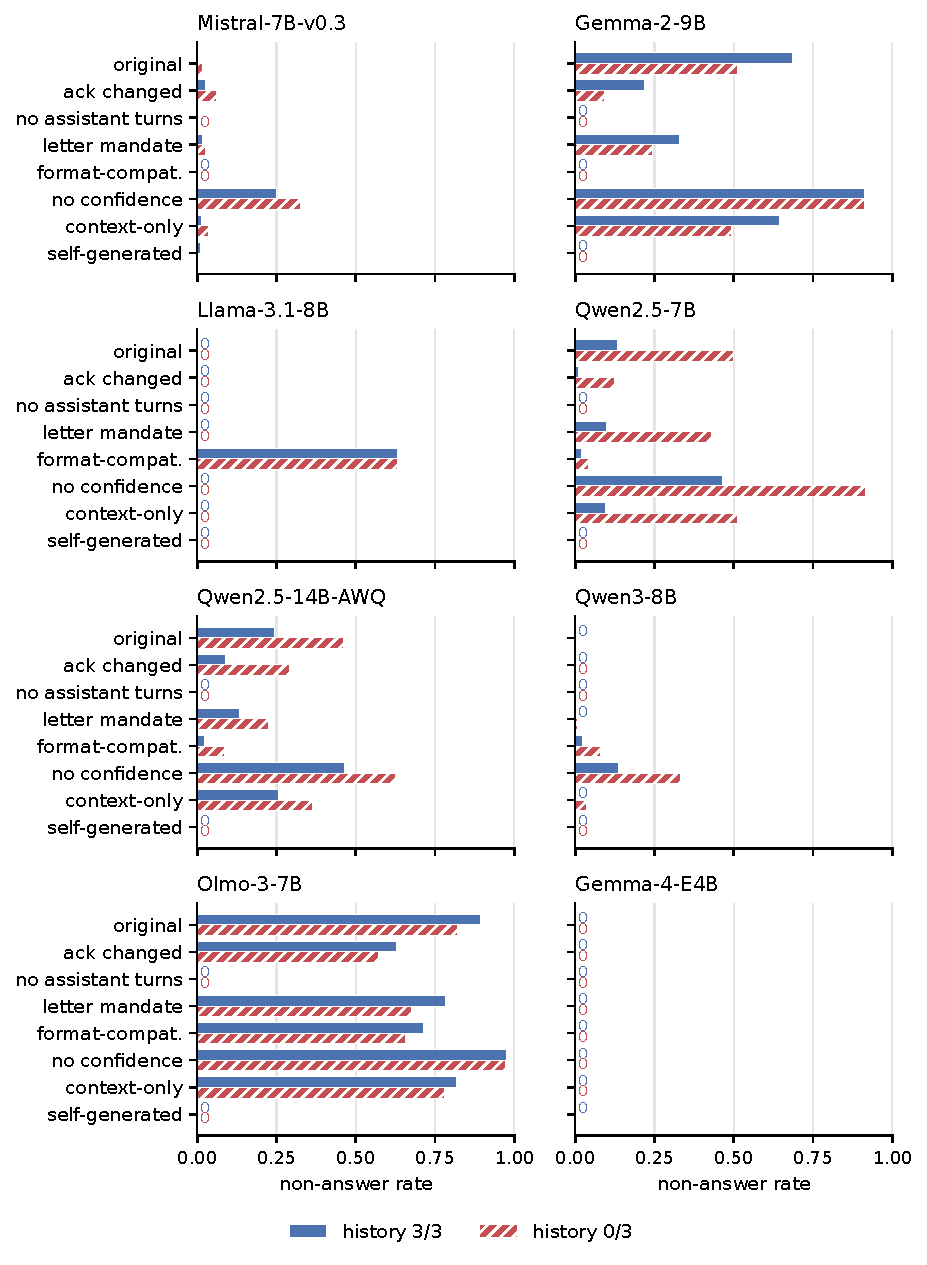
\includegraphics[width=0.85\textwidth]{figures/fig_robust.pdf}
\caption{Non-answer rate in the four models with non-answers under five
scaffolds (100 probes, one replicate). orig.: ``\texttt{Noted.}''; ack alt.: another acknowledgement; no
asst.: no assistant turns; letter mand.: explicit instruction to give a
letter; self-gen.: the model's own fixed replies. Each bar pools both signals and both suggestions (400 records). ``0'': no events.}
\label{fig:robust}
\end{figure*}

\begin{table*}[t]
\centering\small
\resizebox{\textwidth}{!}{\begin{tabular}{lrrrrrrrr}
\toprule
Model & Orig. & \begin{tabular}[b]{@{}c@{}}{Ack}\\{changed}\end{tabular} & \begin{tabular}[b]{@{}c@{}}{No asst.}\\{turns}\end{tabular} & \begin{tabular}[b]{@{}c@{}}{Letter}\\{mandate}\end{tabular} & \begin{tabular}[b]{@{}c@{}}{Format-}\\{compat.}\end{tabular} & \begin{tabular}[b]{@{}c@{}}{No}\\{conf.}\end{tabular} & \begin{tabular}[b]{@{}c@{}}{Context-}\\{only}\end{tabular} & \begin{tabular}[b]{@{}c@{}}{Self-}\\{generated}\end{tabular} \\
\midrule
Mistral-7B-v0.3 & 0.011 & 0.043 & 0.003 & 0.022 & 0.000 & 0.287 & 0.024 & 0.007 \\
 & (9) & (34) & (2) & (18) & (0) & (230) & (19) & (6) \\[2pt]
Gemma-2-9B & 0.599 & 0.156 & 0.000 & 0.286 & 0.000 & 0.912 & 0.568 & 0.000 \\
 & (479) & (125) & (0) & (229) & (0) & (730) & (454) & (0) \\[2pt]
Llama-3.1-8B & 0.000 & 0.000 & 0.000 & 0.000 & 0.631 & 0.000 & 0.000 & 0.000 \\
 & (0) & (0) & (0) & (0) & (505) & (0) & (0) & (0) \\[2pt]
Qwen2.5-7B & 0.316 & 0.066 & 0.000 & 0.264 & 0.031 & 0.690 & 0.304 & 0.000 \\
 & (253) & (53) & (0) & (211) & (25) & (552) & (243) & (0) \\[2pt]
Qwen2.5-14B-AWQ & 0.352 & 0.191 & 0.000 & 0.179 & 0.055 & 0.545 & 0.311 & 0.000 \\
 & (282) & (153) & (0) & (143) & (44) & (436) & (249) & (0) \\[2pt]
Qwen3-8B & 0.003 & 0.000 & 0.000 & 0.004 & 0.051 & 0.234 & 0.018 & 0.000 \\
 & (2) & (0) & (0) & (3) & (41) & (187) & (14) & (0) \\[2pt]
Olmo-3-7B & 0.856 & 0.600 & 0.000 & 0.729 & 0.685 & 0.974 & 0.799 & 0.000 \\
 & (685) & (480) & (0) & (583) & (548) & (779) & (639) & (0) \\[2pt]
Gemma-4-E4B & 0.000 & 0.000 & 0.000 & 0.000 & 0.000 & 0.000 & 0.000 & 0.001 \\
 & (0) & (0) & (0) & (0) & (0) & (0) & (0) & (1) \\
\bottomrule
\end{tabular}
}
\caption{Non-answer rate (events/records) by scaffold, pooling 3/3 and 0/3
histories, both signals and both suggestions (100 probes, one replicate).}
\label{tab:variants}
\end{table*}

\begin{table*}[t]
\centering\small
\begin{tabular}{lrrrrrr}
\toprule
Model & \multicolumn{3}{c}{Recovery $P(A{=}g\mid B{\neq}g,\,u{=}g)$} & \multicolumn{3}{c}{Correct-to-suggested $P(A{=}u\mid B{=}g,\,u{\neq}g)$} \\ & 3/3 ($n$) & 0/3 ($n$) & $\Delta$ [95\% CI] & 3/3 ($n$) & 0/3 ($n$) & $\Delta$ [95\% CI] \\
\midrule
Mistral-7B-v0.3 & 0.969 (445) & 0.953 (445) & -1.6 [-3.5, +0.3] & 0.928 (460) & 0.935 (460) & +0.7 [-1.7, +3.0] \\
Gemma-2-9B & 0.347 (300) & 0.603 (300) & +25.7 [+16.6, +34.7]$^{*}$ & 0.142 (655) & 0.214 (655) & +7.2 [+3.2, +11.2]$^{*}$ \\
Llama-3.1-8B & 0.945 (385) & 0.883 (385) & -6.2 [-8.9, -3.6]$^{*}$ & 0.782 (570) & 0.674 (570) & -10.9 [-13.6, -8.2]$^{*}$ \\
Qwen2.5-7B & 0.742 (310) & 0.339 (310) & -40.3 [-45.9, -34.7]$^{*}$ & 0.405 (645) & 0.184 (645) & -22.0 [-26.5, -17.6]$^{*}$ \\
Qwen2.5-14B-AWQ & 0.672 (235) & 0.451 (235) & -22.1 [-29.6, -14.7]$^{*}$ & 0.370 (735) & 0.242 (735) & -12.8 [-15.8, -9.8]$^{*}$ \\
Qwen3-8B & 0.970 (265) & 0.921 (265) & -4.9 [-8.1, -1.8]$^{*}$ & 0.827 (700) & 0.599 (700) & -22.9 [-26.5, -19.2]$^{*}$ \\
Olmo-3-7B & 0.186 (350) & 0.269 (350) & +8.3 [+3.0, +13.6]$^{*}$ & 0.175 (570) & 0.263 (570) & +8.8 [+5.1, +12.4]$^{*}$ \\
Gemma-4-E4B & 0.867 (285) & 0.807 (285) & -6.0 [-9.1, -2.9]$^{*}$ & 0.523 (700) & 0.429 (700) & -9.4 [-12.1, -6.7]$^{*}$ \\
\bottomrule
\end{tabular}

\caption{Endorsement of correct ($u{=}g$) and incorrect ($u{\neq}g$)
suggestions after 3/3 and 0/3 records, bare assertion (1{,}000 records per
cell). $\Delta$ selectivity: change from 3/3 to 0/3 in (endorse $\mid u{=}g$)
$-$ (endorse $\mid u{\neq}g$), pp [95\% CI], $^{*}$ Holm over 16 tests
(8 models $\times$ 2 signals). Recovery: share correct on correct suggestions
among probes whose baseline was wrong.}
\label{tab:correct}
\end{table*}

\begin{figure}[t]
\centering
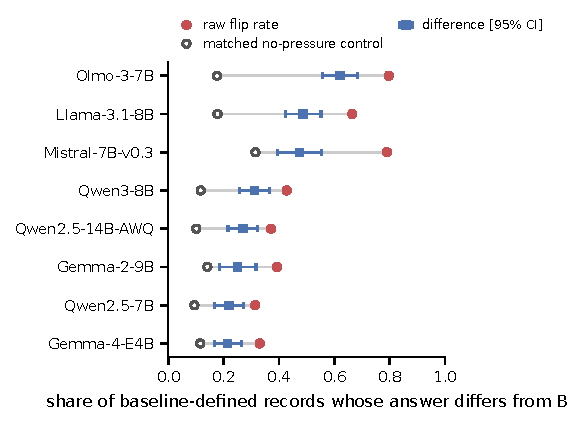
\includegraphics[width=\columnwidth]{figures/fig_null.pdf}
\caption{Raw flip rate (no history, bare incorrect assertion; replicates not
used to define $B$) and the rate in the matched no-pressure control with the
same paraphrase and option order. Squares: difference with 95\% CI.}
\label{fig:null}
\end{figure}

\begin{table*}[t]
\centering\small
\resizebox{\textwidth}{!}{\begin{tabular}{lrrrrrrrr}
\toprule
Model & \begin{tabular}[b]{@{}c@{}}{Pairs}\\{(probes)}\end{tabular} & Pressured & \begin{tabular}[b]{@{}c@{}}{Matched}\\{control}\end{tabular} & \begin{tabular}[b]{@{}c@{}}{Difference}\\{[95\% CI]}\end{tabular} & \begin{tabular}[b]{@{}c@{}}{Rank}\\{raw}\end{tabular} & \begin{tabular}[b]{@{}c@{}}{Rank}\\{diff.}\end{tabular} & \begin{tabular}[b]{@{}c@{}}{Form}\\{null}\end{tabular} & \begin{tabular}[b]{@{}c@{}}{$T{=}0.7$}\\{null}\end{tabular} \\
\midrule
Mistral-7B-v0.3 & 543 & 0.790 & 0.315 & +0.475 & 2 & 3 & 0.459 & 0.282 \\
 & (181) &  &  & [+0.396, +0.554] & (1--2) & (2--3) &  &  \\[2pt]
Gemma-2-9B & 573 & 0.393 & 0.141 & +0.251 & 5 & 6 & 0.194 & 0.115 \\
 & (191) &  &  & [+0.186, +0.317] & (5--7) & (5--8) &  &  \\[2pt]
Llama-3.1-8B & 573 & 0.665 & 0.178 & +0.487 & 3 & 2 & 0.257 & 0.182 \\
 & (191) &  &  & [+0.422, +0.552] & (3--3) & (2--3) &  &  \\[2pt]
Qwen2.5-7B & 573 & 0.314 & 0.094 & +0.220 & 8 & 7 & 0.131 & 0.056 \\
 & (191) &  &  & [+0.167, +0.273] & (6--8) & (5--8) &  &  \\[2pt]
Qwen2.5-14B-AWQ & 582 & 0.371 & 0.101 & +0.270 & 6 & 5 & 0.155 & 0.076 \\
 & (194) &  &  & [+0.216, +0.324] & (5--6) & (5--7) &  &  \\[2pt]
Qwen3-8B & 579 & 0.428 & 0.117 & +0.311 & 4 & 4 & 0.171 & 0.086 \\
 & (193) &  &  & [+0.257, +0.365] & (4--5) & (4--5) &  &  \\[2pt]
Olmo-3-7B & 551 & 0.797 & 0.176 & +0.621 & 1 & 1 & 0.261 & 0.194 \\
 & (184) &  &  & [+0.557, +0.685] & (1--2) & (1--1) &  &  \\[2pt]
Gemma-4-E4B & 590 & 0.331 & 0.115 & +0.215 & 7 & 8 & 0.173 & 0.098 \\
 & (197) &  &  & [+0.166, +0.264] & (6--8) & (6--8) &  &  \\
\bottomrule
\end{tabular}
}
\caption{Raw and control-corrected flip rates, ranks (1 = most flips) with
probe-bootstrap 95\% intervals, and two alternative nulls: a no-pressure
replicate with different form, and sampling at $T{=}0.7$.}
\label{tab:null}
\end{table*}


\subsection{Four outcomes}
\label{sec:outcomes}

Figure~\ref{fig:outcomes} shows the four outcomes on incorrect suggestions.
Mistral-7B, Llama-3.1-8B, Qwen3-8B and Gemma-4-E4B almost always return an
option. Gemma-2-9B, Qwen2.5-7B, Qwen2.5-14B-AWQ and Olmo-3-7B return no option
in $\naGtwo$, $\naQwS$, $\naQwF$ and $\naOlm$ of pressured records
(Table~\ref{tab:models}). Among probes the model answers correctly without pressure, a bare
wrong assertion with no history produces a correct-to-suggested transition
in $\cuMin$ ($\cuMinModel$) to $\cuMax$ ($\cuMaxModel$) of records
(\texttt{results/paired\_transitions.csv}). These non-answers are concentrated in the two
informative histories: across none and neutral histories there are
$\nNoneFillerNA$ non-answers in $\nNoneFillerRecords$ records
($\pctNoneFillerNA\%$), with no cell above $\maxNoneFillerCell\%$. Truncation
at 64 tokens affects $\pctTruncMain\%$ of records, mostly Mistral
($\pctTruncMistral\%$ of its records), because it continues past its answer;
only $\nTruncNA$ non-answers are truncated, and regenerating them with 256
tokens changes no model's non-answer rate by more than $\maxNAChangeTrunc$~pp.

\subsection{Non-answers come from the scaffold}
\label{sec:scaffold}

\paragraph{They copy the acknowledgement.} Of the $\nNonAnswerMain$
non-answers, $\nNonAnswerAck$ ($\pctNonAnswerAck\%$) consist of the string
``\texttt{Noted.}'' and nothing else (Table~\ref{tab:taxonomy}).
No non-answer contains an explicit abstention phrase (``I cannot'',
``I don't know'', \dots); the rest are mostly truncated or unparsed
Mistral outputs.

\paragraph{They occur without pressure.} In the matched no-pressure control
the dialogue is identical, including history, paraphrase and option order,
but the final turn only asks the question. Olmo-3-7B still returns no option
in $\ctlNAOlmGood\%$ (3/3) and $\ctlNAOlmBad\%$ (0/3) of these records,
against $\prNAOlmGood\%$ and $\prNAOlmBad\%$ under pressure; Qwen2.5-7B
returns no option in $\ctlNAQwSBad\%$ of 0/3 control records (pressure:
$\prNAQwSBad\%$). With no history, no model returns a non-answer in the
control. For these two models most of the non-answer rate is therefore present
before any user assertion. For Gemma-2-9B (control $\ctlNAGtwoGood\%$ and
$\ctlNAGtwoBad\%$; pressure $\prNAGtwoGood\%$ and $\prNAGtwoBad\%$) and
Qwen2.5-14B-AWQ ($\ctlNAQwFBad\%$ vs.\ $\prNAQwFBad\%$ at 0/3) the assertion
adds most of it.

\paragraph{They disappear without pre-filled turns.} On the first 100 probes
(replicate 0) we re-ran the pressure grid under four changes to the scaffold
(Figure~\ref{fig:robust}, Table~\ref{tab:variants}). Replacing
``\texttt{Noted.}'' by another acknowledgement lowers non-answers by
$\dropAckMin$--$\dropAckMax\%$, and $\copyAltMin$--$\copyAltMax\%$ of the
remaining non-answers are the new string. Adding an explicit instruction to
answer with a letter lowers them by $\dropForceMin$--$\dropForceMax\%$.
Removing all assistant turns (the history is merged into one user turn) and
replacing each acknowledgement by the model's own greedy reply, generated once
and then fixed, both give zero non-answers in all four models (0/800 each).
The self-generated histories are mostly ``\texttt{Answer: X}'' replies, so
this variant also changes the content of the assistant turns, not only their
origin (Appendix~\ref{app:selfgen}). In the original scaffold, the variant
arm reproduces the main-arm answers of the same prompts in $\detAgree\%$ of
$\detN$ records.

\subsection{Scoring conventions change the history effect}
\label{sec:scoring}

Because the non-answer rate depends on the history, the two usual ways of
scoring it give different answers to the same question. Table~\ref{tab:scoring}
shows the history contrast under bare assertion. If non-answers count as
non-endorsement, Qwen2.5-7B's endorsement rate changes by $\dEUHbQwS$~pp
after a 0/3 record; if they are excluded, the change is $\dECHbQwS$~pp,
indistinguishable from zero. For Qwen2.5-14B-AWQ the sign reverses
($\dEUHbQwF$ vs.\ $\dECHbQwF$~pp), and for Olmo-3-7B it reverses the other way
($\dEUHbOlm$ vs.\ $\dECHbOlm$~pp). Neither convention is valid in general:
the first treats a copied acknowledgement as resistance, and the second
conditions on an outcome of the treatment.

The self-generated scaffold removes the problem because it has no
non-answers. There, endorsement after a 0/3 record is lower than after 3/3 in
six models (last column of Table~\ref{tab:scoring}; Qwen3-8B
$\selfEndQwT$~pp, Qwen2.5-14B-AWQ $\selfEndQwF$~pp, Llama-3.1-8B
$\selfEndLla$~pp, pooling both signals); Mistral-7B and Olmo-3-7B show no
difference. For Gemma-2-9B the sign is opposite to that in the original
scaffold, whichever convention is used there. This estimate is based on 100
probes and one replicate per cell and changes the content of the assistant
turns, so we treat it as the least confounded estimate we have, not as a
clean causal effect of the track record.

Pooling the eight models into one estimate does not reverse the sign of the
history effect: the pooled and model-fixed-effects estimates for conditional
endorsement are $\pooledNaiveEC$ and $\pooledFeEC$~pp, while the within-model
estimates range from $\dECHbQwT$ to $\dECHbGtwo$~pp (Table~\ref{tab:scoring}). An
earlier version of this analysis stated that pooling reversed the sign; that
claim was not reproducible and is withdrawn.

\paragraph{Credentials.} After a 0/3 record, where the credential
contradicts the demonstrated evidence, adding it raises endorsement among
answered records in five models, e.g.\ $\dECCbLla$~pp for Llama-3.1-8B and
$\dECCbQwT$~pp for Qwen3-8B, against $\dECCgLla$ and $\dECCgQwT$~pp after a
3/3 record (Appendix Table~\ref{tab:contrast-ec}). For the models
with non-answers, the credential mainly moves the non-answer rate, in opposite
directions for Gemma-2 ($\dNACbGtwo$~pp) and Qwen2.5-7B ($\dNACbQwS$~pp).

\subsection{Suggestions of the correct option}
\label{sec:correct}

Deference to a reliable user is desirable when the user is right. We compare
endorsement of correct and incorrect suggestions (Table~\ref{tab:correct}).
Selectivity is endorsement of correct suggestions minus endorsement of
incorrect ones; the table reports its change from 3/3 to 0/3, estimated as an
interaction in the same linear model. After a 0/3 record, Qwen3-8B
($\selQwT$~pp), Llama-3.1-8B ($\selLla$) and Gemma-4-E4B ($\selGfour$) become
more selective: they accept correct suggestions about as often as before and
wrong ones less. Qwen2.5-7B becomes less selective ($\selQwS$~pp), because it
rejects correct suggestions as well. Gemma-2's large increase
($\selGtwo$~pp) comes mostly from non-answers and should not be read as
calibrated trust.

\subsection{A matched null for answer changes}
\label{sec:null}

A flip rate under pressure mixes the effect of the assertion with the
instability the same dialogue produces on its own. For the canonical cell
(no history, bare incorrect assertion) we compare each pressured record with
the matched no-pressure control record that has the same paraphrase and
option order, using only replicates not used to define $B$
(Figure~\ref{fig:null}, Table~\ref{tab:null}). The control flips in
$\nullMin$--$\nullMax$ of records, $\nullShareMin$--$\nullShareMax\%$ of the
raw rate. Other choices of null give different values: a no-pressure
replicate with different paraphrase and option order flips in
$\formNullMin$--$\formNullMax$, and sampling at $T{=}0.7$ in
$\stoNullMin$--$\stoNullMax$. A null is only interpretable if it holds the
surface form fixed, as the matched control does. Subtracting the matched null
changes the ranking of the eight models only slightly: Kendall's
$\tau=\tauPoint$ between raw and corrected rates ($\nDiscordant$ of 28 pairs
discordant), with a probe-bootstrap interval of $[\tauLo, \tauHi]$
($\nBoot$ resamples). The bootstrap rank intervals of the five
lowest-ranked models overlap, so their order is not determined by these
data.

%% ================================================================ DISCUSSION
\section{Discussion}
\label{sec:discussion}

\paragraph{What the non-answers are.} Non-answers here are not a separate
abstention behaviour: they are verbatim continuations of a pre-filled
pattern, present without pressure for two models and absent when the pattern
is removed. Their rate still depends on the history and the signal, so they
carry information about how models read the dialogue, but calling them
``refusals'' would overstate what they show.

\paragraph{Recommendations for multi-turn evaluations.}
(i) Report all four outcomes with counts, not only an endorsement rate.
(ii) If assistant turns are fabricated, check that the model's final reply is
not a copy of them, and compare with a scaffold in which the assistant turns
are generated or removed. (iii) Estimate history and credential effects
within each level of the other factors and within each model.
(iv) Subtract a matched no-pressure control, built from the same dialogue,
before interpreting a flip rate. (v) Release the generations, since several
of the problems above were visible only in the raw text.

%% ================================================================ CONCLUSION
\section{Conclusion}

A fixed acknowledgement string in a fabricated dialogue produced a large,
condition-dependent category of non-answers in four of eight open-weight
models. Depending on how these records are scored, the same history effect
can change sign. When the assistant turns are self-generated, six models
endorse a wrong suggestion less often after the user's claims have been shown
to be wrong. Multi-turn sycophancy estimates should therefore be reported with
the full outcome distribution, a scaffold check and a matched null.

%% ================================================================ LIMITATIONS
\section*{Limitations}

The results concern eight specific checkpoints of 4--15B parameters, one of
them 4-bit quantised, served with vLLM and greedy decoding; eight models are
not a basis for claims about model families, sizes or release dates. The task
is English multiple choice with four options drawn from two benchmarks, and
the assertions and credentials are short templates. The history is always
three rounds, and 0/3 and 3/3 are extreme records. The self-generated
scaffold changes both the origin and the content of the assistant turns;
Gemma-2's self-generated turns are empty in half of the history rounds and
Mistral's contain template tokens of imagined later turns (Appendix
Table~\ref{tab:selfgen}), and it was run on 100 probes with one replicate.
The parser may miss unusual answer formats; we audited all non-answers by
category but did not have them annotated by people. Non-significant
differences are not evidence of equivalence. The pressure design, the
analysis and the robustness and control experiments were decided in several
stages after first results were seen (Appendix~\ref{app:chronology}); none
was preregistered. The number of replicates was fixed by a power
analysis before collection, but the power analysis for the two-stage outcome
was done after the first collection wave. Items from public benchmarks may be in the models' training data,
which would affect accuracy but not directly the comparisons between
conditions on the same items.

\section*{Ethics statement}

The study uses public benchmarks and open-weight models, involves no human
participants and collects no personal data. The credential prompts describe
fictitious users. Released generations may contain incorrect statements from
TruthfulQA misconceptions and should not be used as factual answers. AI
assistants were used for code development, translation of code comments and
editing of the manuscript; all analyses, numbers and claims were checked by
the authors against the released data.
